\documentclass[fontsize = 10pt, paper= a4]{jlreq}

\usepackage[dvipdfmx]{graphicx}
\usepackage{color}
\usepackage{listings}
\usepackage{url}
\definecolor{OliveGreen}{rgb}{0.0,0.6,0.0}
\definecolor{Magenta}{cmyk}{0, 1, 0, 0}
\definecolor{colFunc}{rgb}{1,0.07,0.54}
\definecolor{CadetBlue}{cmyk}{0.62,0.57,0.23,0}
\definecolor{Brown}{cmyk}{0,0.81,1,0.60}
\definecolor{colID}{rgb}{0.63,0.44,0}
\lstset{
language={C},                   %言語の指定
basicstyle={\ttfamily\small},        %書体の指定
backgroundcolor={\color[gray]{.95}}, %背景色と透過度
keywordstyle={\color{blue}},         %キーワード(int, ifなど)の書体指定
commentstyle={\color{OliveGreen}},   %注釈の書体 
stringstyle=\color{Magenta},         %文字列
frame=single,                        %枠縁(leftline,topline,bottomline,lines,trBL,shadowbox, single)
numbers=left,                        %行番号表示
numberstyle={\ttfamily\small},       %行番号の書体指定
breaklines=true,                     %折り返し(自動改行)
breakindent = 10pt,                  %自動改行後のインデント量(デフォルトでは20[pt])	
tabsize=2,                           %タブの大きさ
captionpos=t                         %キャプションの場所(t,b : "tb"ならば上下両方に記載)
}
\renewcommand{\lstlistingname}{図} % キャプション名の指定

\begin{document}

\title{統計分析法 第8週レポート}
\author{202212022 田島瑞起}
\date{2023/12/12}
\maketitle
\section{設問1-1,1-3}
    week8-data-odd.csvのデータを散布図としてプロットした上に、回帰直線を追加したものが下記の図となる。
    \begin{figure}
        \centering
        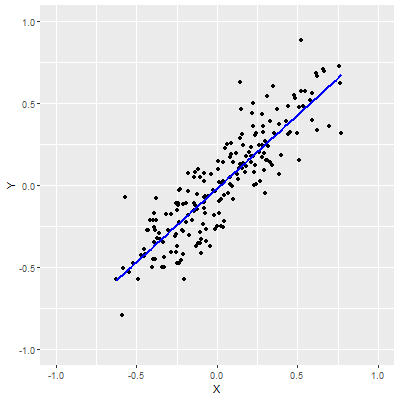
\includegraphics[width=4cm]{8-1.png}
    \end{figure}
    

\section{設問1-2}

\begin{lstlisting}[basicstyle=\ttfamily\footnotesize, frame=single]
    #結果
    Call:
    lm(formula = y ~ x)

    Residuals:
        Min       1Q   Median       3Q      Max 
    -0.37165 -0.10421  0.00426  0.11478  0.51488 

    Coefficients:
                Estimate Std. Error t value Pr(>|t|)    
    (Intercept) -0.01775    0.01116  -1.591    0.113    
    x            0.89836    0.03511  25.588   <2e-16 ***
    ---
    Signif. codes:  0 ‘***’ 0.001 ‘**’ 0.01 ‘*’ 0.05 ‘.’ 0.1 ‘ ’ 1

    Residual standard error: 0.1573 on 198 degrees of freedom
    Multiple R-squared:  0.7678,    Adjusted R-squared:  0.7666 
    F-statistic: 654.7 on 1 and 198 DF,  p-value: < 2.2e-16

    \end{lstlisting}

\section{設問1-4}
    1-2で示したsummaryの値を読み取ると、回帰直線の傾きaは0.89836、切片bは-0.01775、残差標準偏差0.1573、
    自由度については回帰の自由度: 1残差の自由度: 198、データ数200、決定係数0.7678であることが分かる。

\section{設問1-5}
    今回のデータセットでは相関係数が0.8762453 でありこの値は決定係数の0.7678と近しい値であることが分かる。
    この二つの係数に直接的な数式の関係があるわけではないが、近しい値をとったことには理由が存在し、
    それは相関係数が二つの変数がどれだけ強く関係しているか示す値であり、
    一方決定係数は回帰モデルがデータをどれほど正確に表現しているかを表す値であるからと考えられる。
    今回の場合はデータが直線に近い形であったため、相関係数は1に近い値をとり、回帰モデルによってデータの集合を表現することに問題がなかったため、
    両者の値が高くなったと考えることが出来る。
   
\section{設問1-6}
    相関係数が0.8762453であり、また残差標準偏差0.1573,決定係数が0.7678であることから、この回帰直線はデータを良く反映していると判断することが出来るため、
    xとyには正の相関関係があると判断することが出来る。

\section{設問2-1}
帰無仮説を「得点は教科ごとに差がない」、有意水準0.05としてaov検定を行う。
学生と科目に対応がない場合のaov分析の結果は下記の図の通りとなった。
p値が優位水準を下回るため、帰無仮説は棄却され、得点は教科ごとに差があると結論付けることが出来る。
また分散説明率を計算すると0.9997588と算出された。よってモデルがデータの変動をよく説明していることを示している


\begin{lstlisting}[basicstyle=\ttfamily\footnotesize, frame=single]

    Df Sum Sq Mean Sq F value  Pr(>F)   
sub          2   3344  1671.8   5.618 0.00593 **
Residuals   57  16962   297.6                   
---
Signif. codes:  0 ‘***’ 0.001 ‘**’ 0.01 ‘*’ 0.05 ‘.’ 0.

    \end{lstlisting}

\section{ソースコード}
\begin{lstlisting}[basicstyle=\ttfamily\footnotesize, frame=single]
    #課題1

#データの下準備
setwd('Z:/stats_work')
Data <- read.csv("week8-data-odd.csv")
x <- Data$X
y <- Data$Y

#散布図の描画
library(ggplot2)
plot <- ggplot(Data, aes(x = X, y = Y)) +
  geom_point() +
  xlim(-1.0, 1.0) +
  ylim(-1.0, 1.0)

#散布図に回帰直線を追加した後に画像化
model <- lm(Y ~ X, data = Data)
png("8-1.png", width = 400, height = 400)
plot + geom_smooth(method = "lm", se = FALSE, color = "blue")
dev.off()

#相関係数を求める
Correlation <- cor.test(x,y,method="pearson")

# 単回帰分析の実行
model <- lm(y ~ x)

# 回帰結果の表示
summary(model)

#課題2

# データの読み込み
load("effect-example.dat")

# aov関数を用いた分散分析
model <- aov(score ~ sub, data = scoreDataES)

# 結果の表示
summary(model)

# 分散分析の結果から必要な情報を取得
SS_total <- sum((scoreDataES$score - mean(scoreDataES$score))^2)
SS_residual <- sum(residuals(model)^2)

# 分散説明率の計算
variance_explained <- (SS_total - SS_residual) / SS_total * 100

# 結果の表示
cat("Variance Explained:", variance_explained, "%\n")
    \end{lstlisting}
\end{document}